\subsection{Vue d'ensemble}

L'OMEGAAA possède plusieurs composants que l'ont peut regrouper en quatre
catégories en plus du microcontroleur : les capteurs, les composants de stockage,
les témoins et les composants de communication.\\

Le microcontroleur est le cerveau de l'OMEGAAA. Il possède le programme
informatique, les moyens pour l'exécuter et gérer les autres composants électroniques.
l'un des concepts clé utilisé dans le microcontroleur est sa capacité à effectuer des
échanges d'informations entre les composants par DMA \footnote{DMA : \textbf{D}irect
\textbf{M}emory \textbf{A}cces. Avec la communication par DMA, le microcontrôleur
peut déléguer la tâche de transfert de données à un contrôleur DMA dédié. Le contrôleur
DMA est capable de transférer les données directement entre les périphériques (par exemple,
entre un capteur) et la mémoire de l'ordinateur sans passer par le CPU. Cela libère le
temps CPU pour qu'il puisse effectuer d'autres tâches.}. Le projet OMEGAAA se base sur
l'utilisation d'un STM32F411CEx.\\

Les différents capteurs sont :
\begin{itemize}
    \item Un IMU (Inertial Measurement Unit) qui mesure l'accélération de
    translation et la vitesse de rotation de la fusée (ref: BMI088).
    \item Un GPS qui mesure la position de la fusée et sa vitesse (ref: MAX-M10Q).
    \item Un baromètre qui mesure l'altitude de la fusée et un thermomètre.
    (ref: BMP388).\\
\end{itemize}

\begin{minipage}{0.95\textwidth}

    \begin{wrapfigure}{R}{0.5\textwidth}
        \vspace{1.4cm}
        \centering
        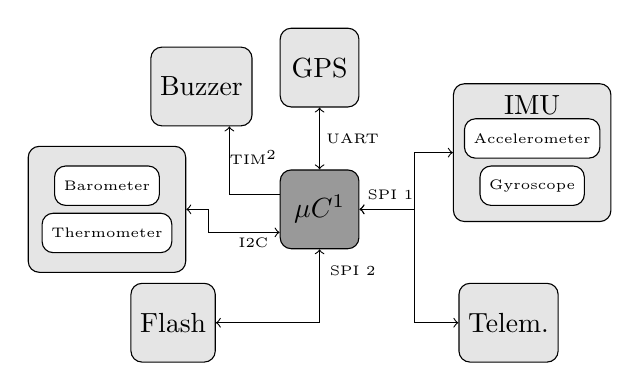
\begin{tikzpicture}[scale=1.2]
    
            \node[draw, rectangle, minimum width=1cm, minimum height=1cm, fill=gray!80, rounded corners]      (micro) at (0, 0) {$\mu C$\footnotemark};
            \node[draw, rectangle, minimum width=2.0cm, minimum height=1.75cm, fill=gray!20, rounded corners] (imu)   at (2.25, +0.60) {};
            \node[draw, rectangle, minimum width=0.5cm, minimum height=0.5cm, fill=white, rounded corners]    (acc)   at (2.25, +0.75) {\tiny Accelerometer};
            \node[draw, rectangle, minimum width=0.5cm, minimum height=0.5cm, fill=white, rounded corners]    (gry)   at (2.25, +0.25) {\tiny Gyroscope};
            \node at (2.25, +1.10) {IMU};
            \node[draw, rectangle, minimum width=1cm, minimum height=1cm, fill=gray!20, rounded corners]      (gps)   at (0, +1.50) {GPS};
            \node[draw, rectangle, minimum width=2.0cm, minimum height=1.60cm, fill=gray!20, rounded corners] (bmu)   at (-2.25, +0.00) {};
            \node[draw, rectangle, minimum width=0.5cm, minimum height=0.5cm, fill=white, rounded corners]    (bar)   at (-2.25, +0.25) {\tiny Barometer};
            \node[draw, rectangle, minimum width=0.5cm, minimum height=0.5cm, fill=white, rounded corners]    (tem)   at (-2.25, -0.25) {\tiny Thermometer};
            \node[draw, rectangle, minimum width=1cm, minimum height=1cm, fill=gray!20, rounded corners]      (tel)   at (+2.00, -1.20) {Telem.};
            \node[draw, rectangle, minimum width=1cm, minimum height=1cm, fill=gray!20, rounded corners]      (mem)   at (-1.55, -1.20) {Flash};
            \node[draw, rectangle, minimum width=1cm, minimum height=1cm, fill=gray!20, rounded corners]      (buz)   at (-1.25, +1.30) {Buzzer};
    
            \draw[<->] (micro) -| ++(1, 0.25) |- (imu);
            \draw[<->] (micro) -- (gps);
            \draw[<->] (micro.-150) -| ++(-0.75, 0.2) |- (bmu);
            \draw[<->] (micro) -| ++(1, -0.25) |- (tel);
            \draw[<->] (micro) |- (mem);
            \draw[->] (micro.160) -| (buz.-55);
    
            \node at (+0.75, 0.15) {\tiny SPI 1};
            \node at (-0.70, -0.35) {\tiny I2C};
            \node at (+0.35, 0.75) {\tiny UART};
            \node at (-0.70, 0.55) {\tiny TIM\footnotemark};
            \node at (+0.35, -0.65) {\tiny SPI 2};
    
        \end{tikzpicture}
        \caption{Schéma des composants de l'OMEGAAA}
        \label{fig:omega}
    \end{wrapfigure}

Un seul composant de stockage est utilisé : une mémoire flash de 16 Mo
(ref: W25Q128JVPQ).

\vspace{0.5cm}

Les témoins sont des composants qui permettent de savoir dans quel état se
trouve l'OMEGAAA. Ils peuvent être sonores ou lumineux. Dans la version actuelle
de l'OMEGAAA, un buzzer passif est utilisé permettant la création de mélodie.

\vspace{0.5cm}

Un seul composant de communication est utilisé, un module de télémétrie par
protocole et modulation LoRa (ref: RFM98W). A noté que le microcontroleur
possède aussi des moyens de communocation interfaçable avec un ordinateur (via
USB).

\vspace{0.5cm}

Un cinquième type de composant pourrait être ajouté : les actionneurs. Ils
permetteraient d'agire physiquement sur des éléments de la fusée. Par exemple,
un servomoteur contrôlant une surface portante.

\end{minipage}

\vspace{0.5cm}

La figure \ref{fig:omega} montre un schéma des composants de l'OMEGAAA et
leurs interconnexions. Les flèches indiquent les protocoles de communication
utilisés entre les composants.\\


\footnotetext{$\mu C$ : \textbf{M}icro\textbf{C}ontroleur.}
\footnotetext{TIM : \textbf{T}imer \textbf{I}nterface \textbf{M}odule sert dans ce contexte à générer des signaux PWM.}